
%%%%%%%%%%%%%%%%%%%%%%% file typeinst.tex %%%%%%%%%%%%%%%%%%%%%%%%%
%
% This is the LaTeX source for the instructions to authors using
% the LaTeX document class 'llncs.cls' for contributions to
% the Lecture Notes in Computer Sciences series.
% http://www.springer.com/lncs       Springer Heidelberg 2006/05/04
%
% It may be used as a template for your own input - copy it
% to a new file with a new name and use it as the basis
% for your article.
%
% NB: the document class 'llncs' has its own and detailed documentation, see
% ftp://ftp.springer.de/data/pubftp/pub/tex/latex/llncs/latex2e/llncsdoc.pdf
%
%%%%%%%%%%%%%%%%%%%%%%%%%%%%%%%%%%%%%%%%%%%%%%%%%%%%%%%%%%%%%%%%%%%


\documentclass[runningheads,a4paper]{llncs}

\usepackage{nomencl}
\usepackage{amssymb}
\usepackage{todonotes}
\setcounter{tocdepth}{3}
\usepackage{graphicx}
\usepackage{enumitem}
\usepackage{url}
%\urldef{\mailsa}\path|{alfred.hofmann, ursula.barth, ingrid.haas, frank.holzwarth,|
%\urldef{\mailsb}\path|anna.kramer, leonie.kunz, christine.reiss, nicole.sator,|
%\urldef{\mailsc}\path|erika.siebert-cole, peter.strasser, lncs}@springer.com|    
\newcommand{\keywords}[1]{\par\addvspace\baselineskip
\noindent\keywordname\enspace\ignorespaces#1}
\usepackage[unicode=true]{hyperref}

\begin{document}

\mainmatter  % start of an individual contribution

% first the title is needed
\title{Brain Speed Reader}
%\vspace{1cm}
% a short form should be given in case it is too long for the running head
\titlerunning{Brain Speed Reader}
%\thanks{Please note that the LNCS Editorial assumes that all authors have used
%the western naming convention, with given names preceding surnames. This determines
%the structure of the names in the running heads and the author index.}


% the name(s) of the author(s) follow(s) next
%
% NB: Chinese authors should write their first names(s) in front of
% their surnames. This ensures that the names appear correctly in
% the running heads and the author index.
%
\author{Thomas, Nick, Benjamin, John}


\authorrunning{Thomas, Nick, Benjamin, John}
%% (feature abused for this document to repeat the title also on left hand pages)
%
%% the affiliations are given next; don't give your e-mail address
%% unless you accept that it will be published
\institute{School of Information,\\
UC Berkeley, Berkeley,\\
United States}
%%\mailsa\\
%%\mailsb\\
%%\mailsc\\
%%\url{http://www.springer.com/lncs}
%\and Chair of Entrepreneurial Risks,\\ ETH Zurich, Switzerland}
%
%%
% NB: a more complex sample for affiliations and the mapping to the
% corresponding authors can be found in the file "llncs.dem"
% (search for the string "\mainmatter" where a contribution starts).
% "llncs.dem" accompanies the document class "llncs.cls".
%

%\toctitle{Lecture Notes in Computer Science}
\tocauthor{Authors' Instructions}
\maketitle

\begin{abstract}
At the age of online information abundance, the human capacity to retain knowledge is largely limited by the time and the attention required to read text, watch videos, listen to podcasts. For written information, rapid serial visual presentation (RSVP) helps greatly save time with similar levels of text understanding, compared with traditional reading. However, RSVP does not account for attention. We present a simple hybrid brain-computer interface (BCI) that controls in real-time the speed of reading by measuring the instant level of higher cognitive brain activity. Electroencephalogram (EEG) signal is acquired with a single channel consumer-grade headset and analyzed in the frequency domain. The pace of word display is controlled by a measure brainwave entropy. We have conducted a controlled experiment with 50 subjects with three distinct treatments, and we show that brain-controlled speed-reading increases the speed and the understanding of texts by subjects.
\end{abstract}
\section{Introduction}
\section{Related Work}

\subsection{RSVP}



\subsection{Brainwaves}




\section{Apparatus}
The brain speed-reader is an apparatus, which displays words on a screen at variable $r(t)$, which in turn is read by the user. The reading task triggers a change of brain activity, which can be recorded and analyzed through electroencephalograms (EEG). As our apparatus is conceived for use in a naturalistic environment, we have used, {\it Neurosky Mindwave}, the cheapest consumer-grade EEG headset available for less than \$100 on the market. As shown on Figure \ref{fig:apparatus} and explained step-by-step below, the EEG signal is processed online, in order to adapt the rate of words displayed as function of cognitive activity: if the rate $r$ is too large (resp. too low) at time $t$, then reading triggers more  (resp. less) cognitive activity, which in turn allows reducing (resp. increasing) $r$ at $t+1$. In this section, we explain step-by-step the design of the apparatus in details.

\begin{figure}[!t]
\centering
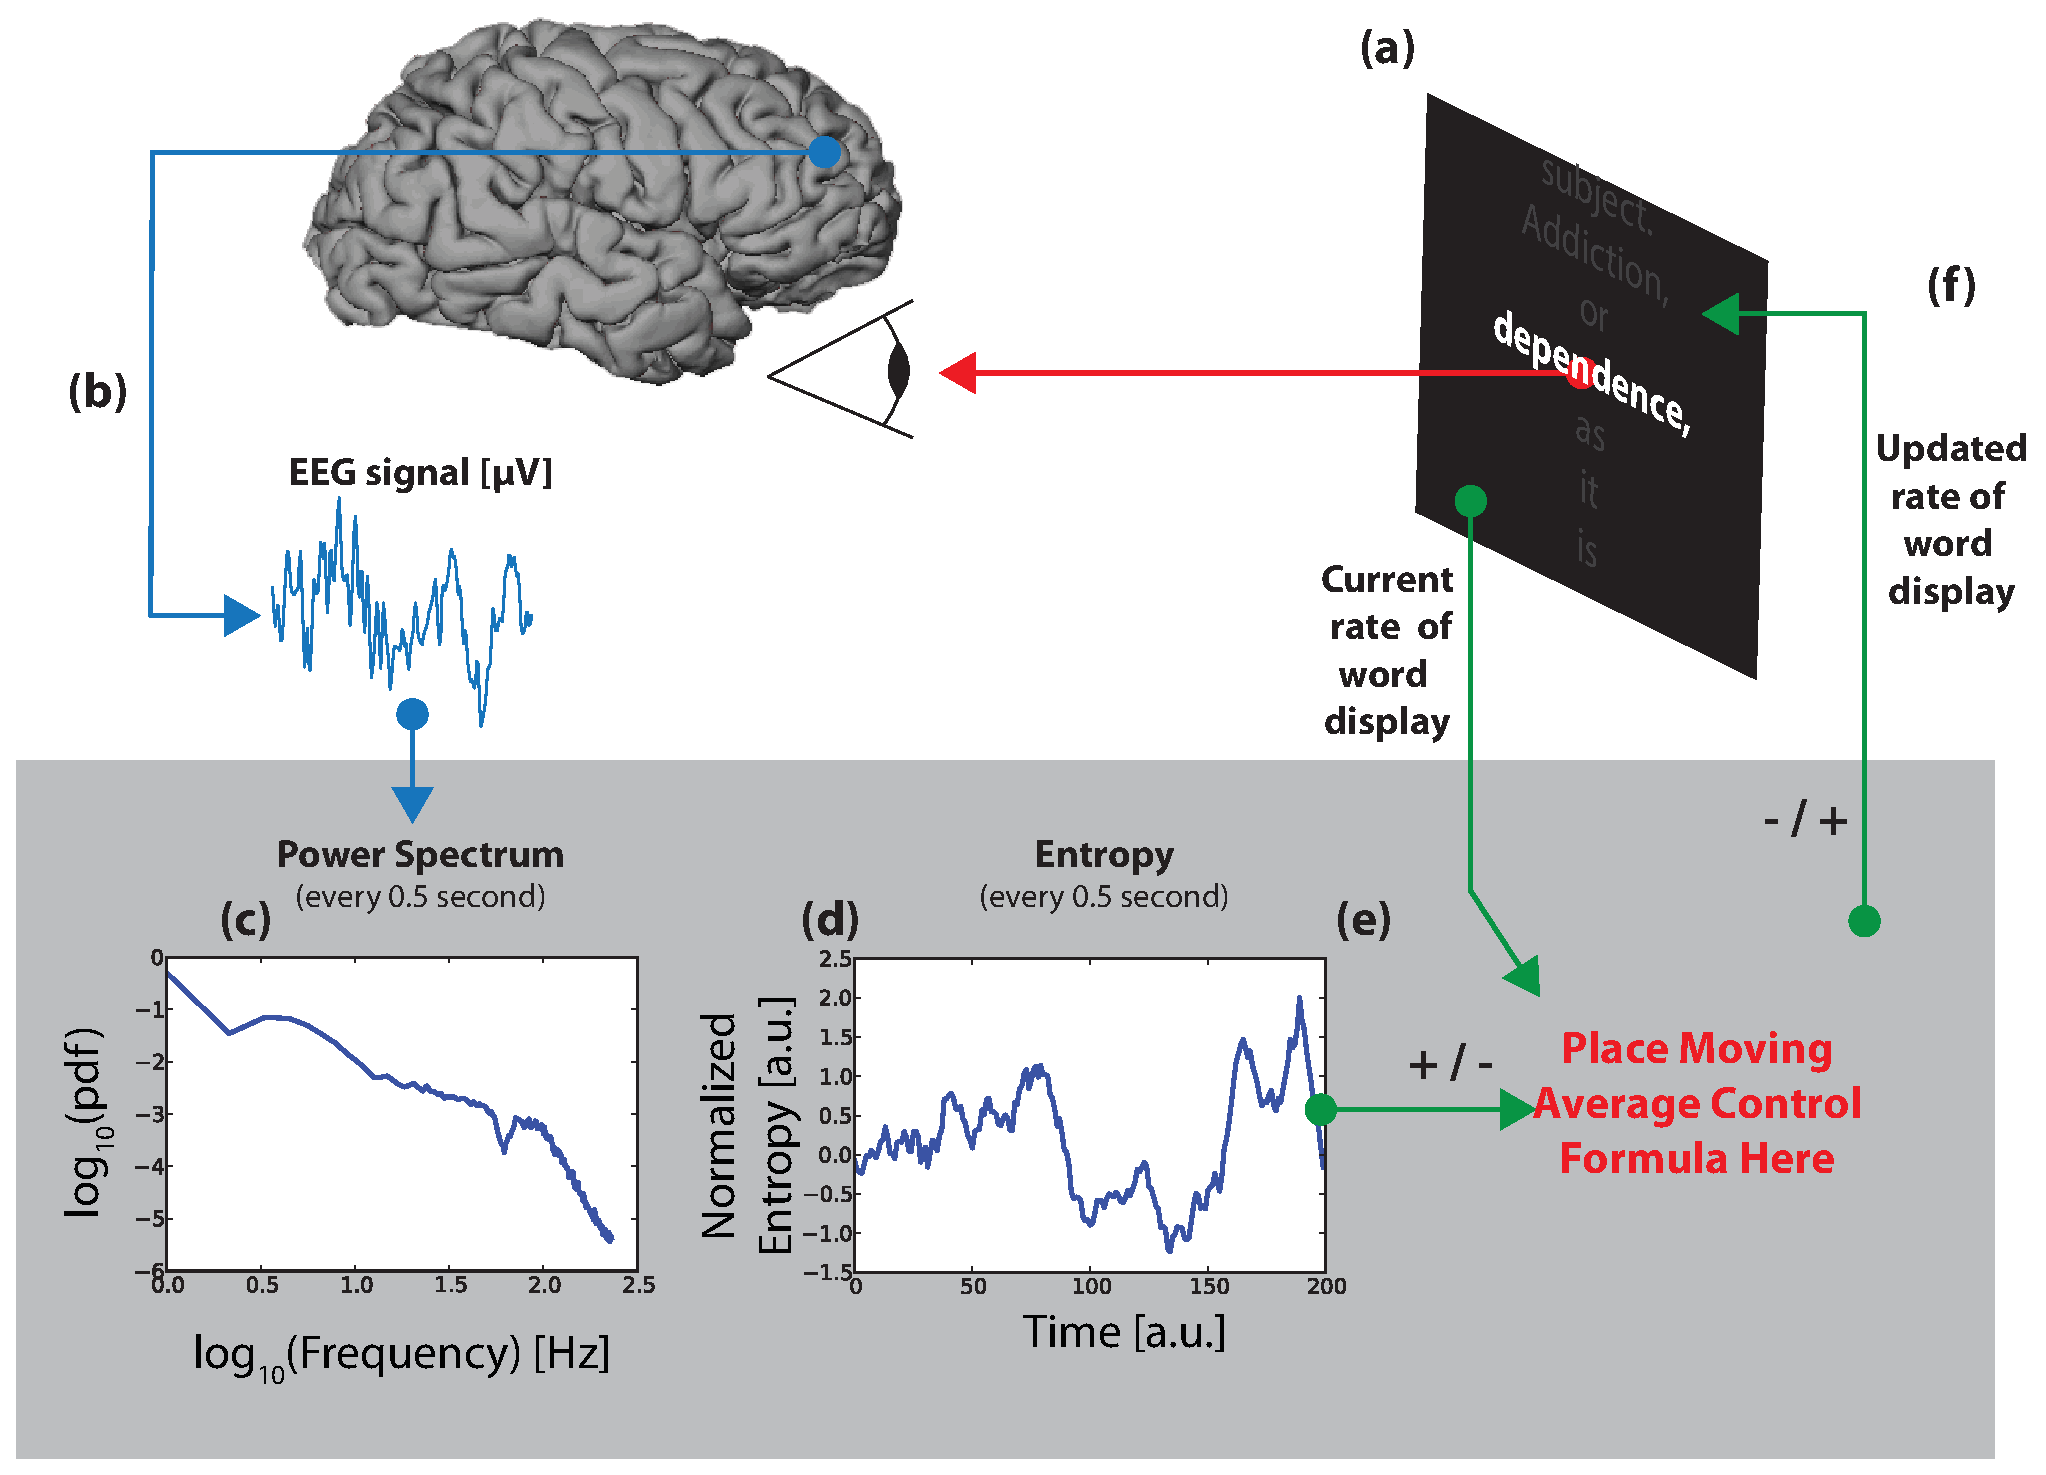
\includegraphics[width=0.9\columnwidth]{../figures/apparatus.eps}
\caption{Brain speed-reader apparatus: {\bf (a)} Words are displayed and read one after the other at a given rate. {\bf (b)} the EEG signal is recorded through a consumer grade device (here the {\it Neurosky Mindwave}). {\bf (c)} The EEG signal is turned every 0.5 seconds into a power spectrum through a Fourier transform, {\bf (d)} the characteristics of the power spectrum are compressed into a single value characteristic entropy $s$ value. {\bf (e)} A new rate of word display is updated by taking into its current value and $s$. {\bf (f)} The rate of word display is updated accordingly.}
\label{fig:apparatus}
\end{figure}

\subsection{Rate of Word Display}
The principle of {\it Rapid Serial Visual Presentation} (RVSP) applied to text, is precisely to display the words of a text at a controlled rate. However, in most RVSP implementations for text, the rate of word display pre-determined and remains constant. In our implementation, the user first calibrates the brain speed-reader by tuning a comfortable baseline word display rate $r_{baseline} = r(t = 0)$. The operation takes only a few seconds. This is a usual way to proceed when using usual text RVSP applications.

\subsection{Brain Activity as Captured by EEG signal}
Unlike traditional text RVSP, we wish to let the user adapt the rate of word display in real-time, through brain activity as captured by EEG signal, to control for a text becoming suddenly becoming more difficult, or just because the mindset of the user has changed, like sudden focus on an important part of the text (lower rate desired) or, on the contrary, loss of attention (higher rate of word displayed desired).

Because we want our apparatus be usable outside the lab, we have chosen the cheapest consumer-grade EEG scanner, available on the market for less than \$100.

\subsection{EEG Signal Processing}
One way to process the EEG signal, consists in analyzing its spectral properties over a determined period. Here, we take a time window of 0.25 second, which allows us to analyze the frequency domain $0-128Hz$, since the sampling rate of the Neurosky Mindwave is 512 measures per second (i.e., 512 Hz). Hence, every 0.25 second, we compute the power spectrum given by, 

 \begin{equation}
\label{eq:pspectrum}
\mathbf{[pspectrum~here]}
\end{equation}
 
and which is expected to approximately follow a power law, i.e., the probability to find a frequency $x$ is given by the probability density function $pdf(x)  = 1/x^{\mu+1}$. The power spectrum varies as a function of the mental tasks occurring, and potential external perturbations, such as voice, imperceptible and perceptible muscle movements, eye-movement, blinking.


\begin{figure}[!t]
\centering
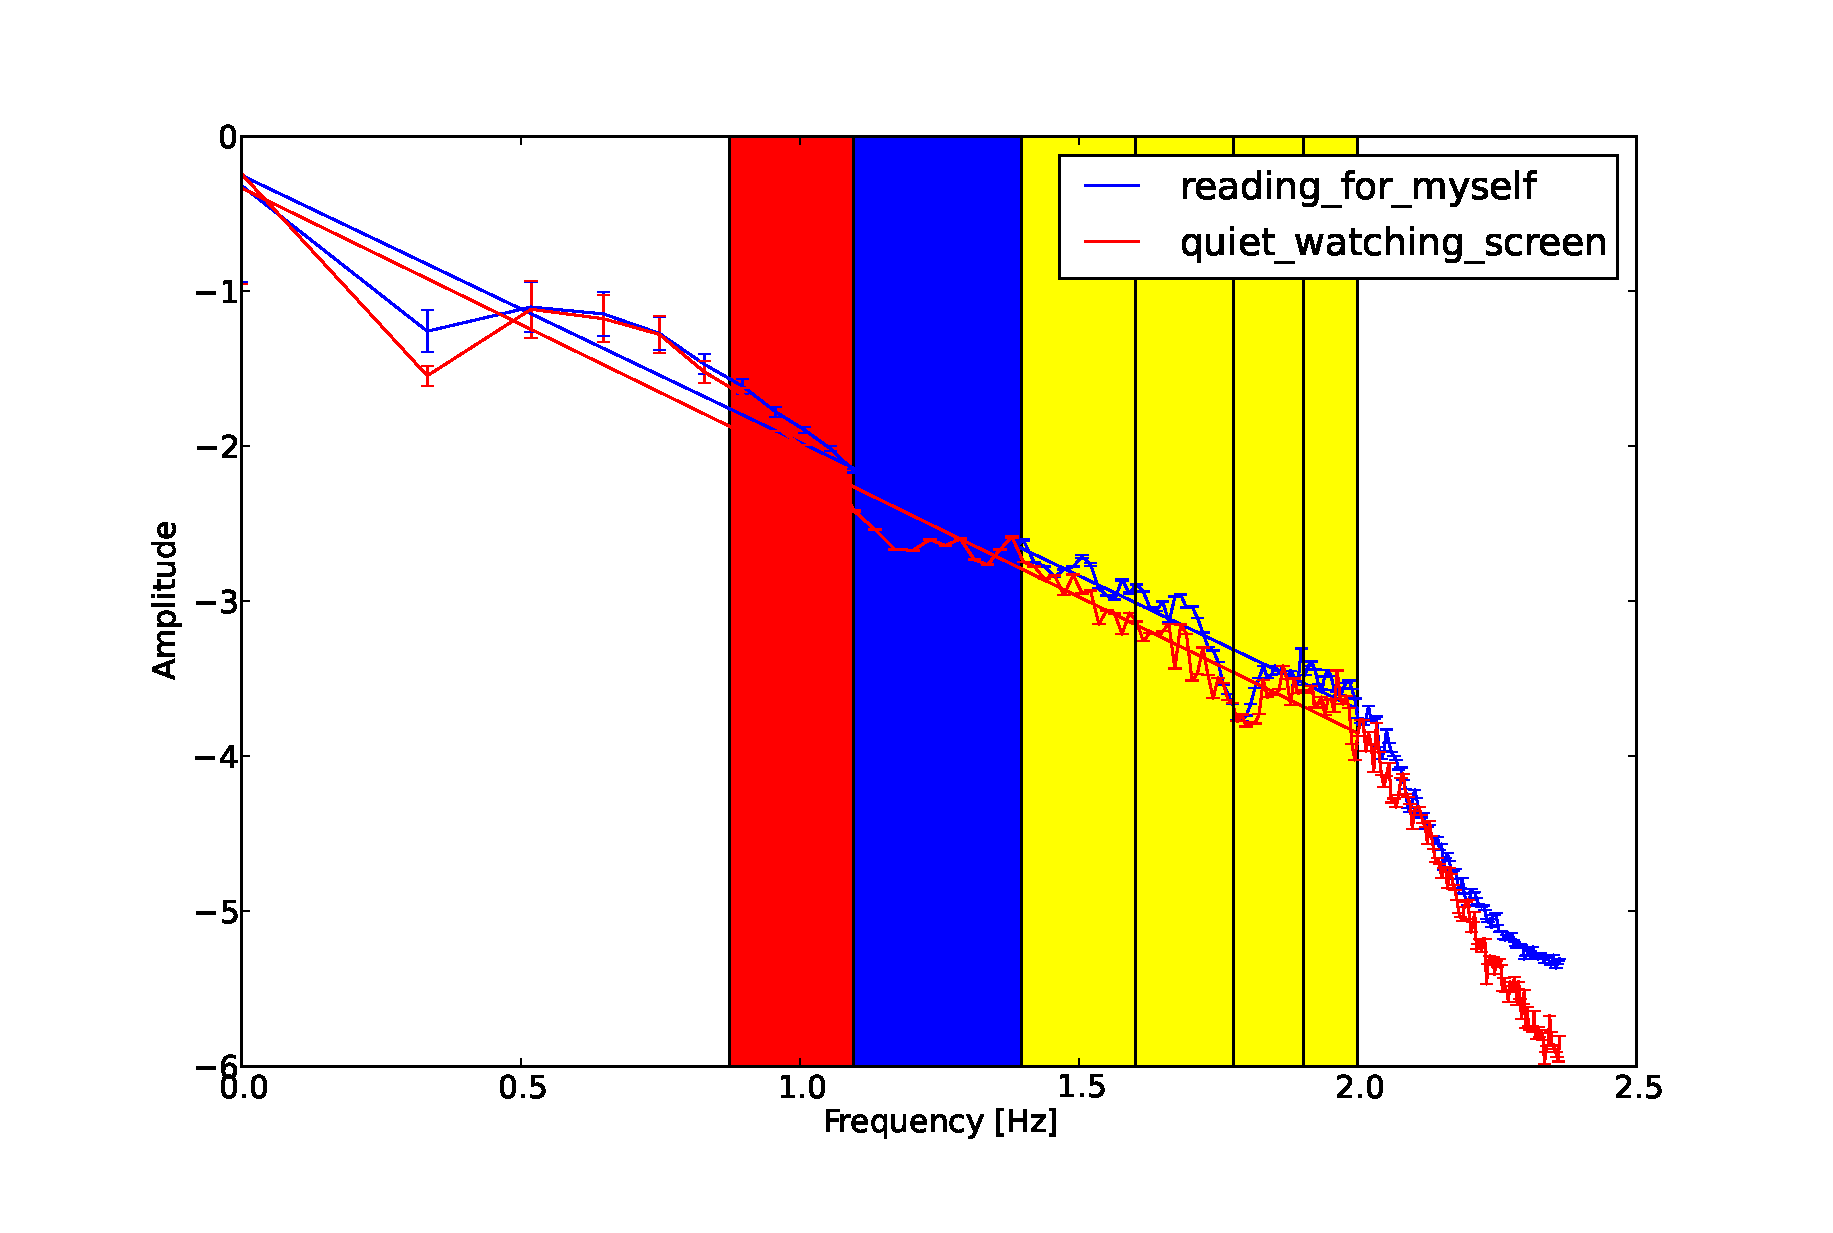
\includegraphics[width=0.9\columnwidth]{../figures/compare_pSpectra.eps}
\caption{Comparison of power spectra of a subject (i) resting state and (ii) reading a text in English for himself. {\bf [report the entropy values in both cases]}}
\label{fig:pspectrum}
\end{figure}


Then, entropy.

\begin{equation}
\label{eq:tsallis}
S_q(X) = \frac{1}{q-1} \left( 1 - \sum_{i=1}^n (p_i)^q \right).
\end{equation}

\begin{equation}
\label{eq:shannon}
S_1(X) = - \sum_{i=1}^n p_i\cdot log_{2}(p_i), ~~for~~q=1.
\end{equation}

\subsubsection{Why Entropy ?}

higher frequencies are usually associated to higher cognitive brain activation. Higher activation  translated into larger entropy $S$.


We wanted a lightweight mobile apparatus, which does not require complicated machine learning or any communication with a cloud service, or would not drain a battery. We purposely decided for a cheap update method {\bf [continue this point in discussion because it helps introduce future work]}

\begin{figure}[!t]
\centering
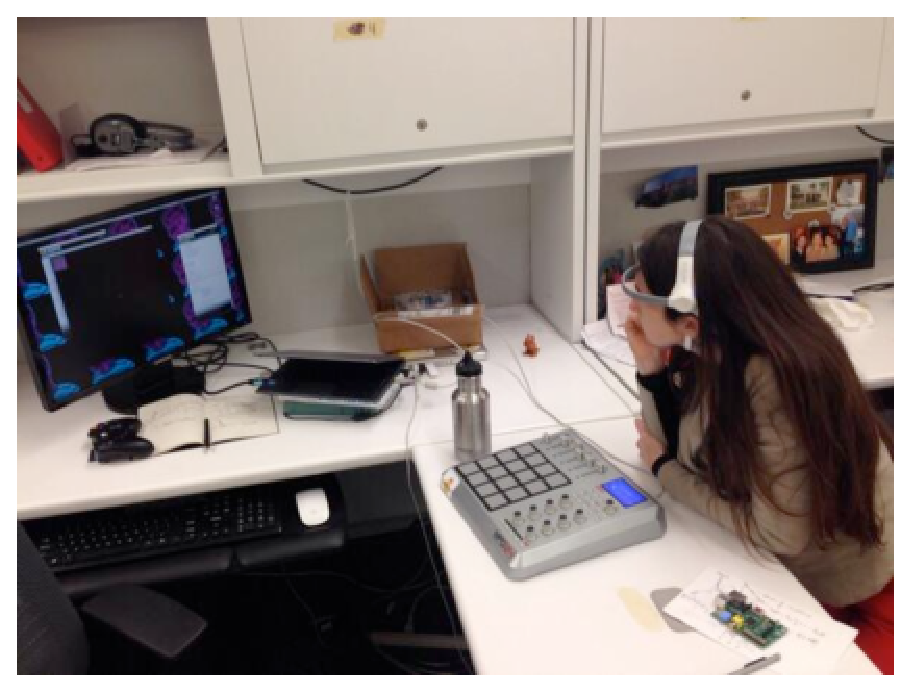
\includegraphics[width=0.9\columnwidth]{../figures/ariel.eps}
\caption{Ariel Garten (Interaxon / Muse CEO) playing with the brain speed reader.}
\label{fig:ariel}
\end{figure}

One could argue that we could have taken the {\it meditation} and {\it attention} metrics provided by Neurosky (and computed directly in the headset). However, these metrics are proprietary and their formula kept secret (we suspect nevertheless that they take $\alpha$ and $\beta$ waves  as an input). Furthermore, extensive testing did not allow us find any consistency with what we would quality meditation or attention. As a result, we preferred to stick to the principles of reproducible science.

\subsection{Negative Feedback Loop}

Explain: higher cog. activity  $\rightarrow$  higher entropy $\rightarrow$  lower word display rate $\rightarrow$ lower cog. activity. {\bf [probably not worth a section]}


\subsection{Word Display Rate Update}

\begin{equation}
\label{eq:Snormalized}
S_{norm}(t) = \frac{S(t) - \langle S \rangle}{\sigma_{S}}, 
\end{equation}
with $\langle S \rangle$ and $\sigma_{S}$ the average and standard deviation of the entropy $S$ calculated over the last 20 points (i.e., the last 5 seconds?). The normalization ensures that $S_{norm}$ is always centered around $0$. The rate $R(t+1)$ of word display is then updated as follows,

\begin{equation}
R(t+\Delta t) = R(t) \left[1 - \alpha \cdot S_{norm}(t)\right],
\label{eq:RateChange}
\end{equation}

where $\Delta t = 0.25$ seconds and $\alpha = 0.20$. In other words, the normalized entropy influences for 20\% the rate change $\Delta R =  \left[ R(t+\Delta t) - R(t) \right] / R(t) = - \alpha \cdot S_{norm}(t)$. Increasing $\alpha$ increases the influence of $S_{norm}$, and the negative sign ensures control of $R$ with a mean reverting process. Note however, that since $S_{norm}$ is calculated from a moving average on a rather short time window, $R$ exhibits excursions (c.f. Figure \ref{fig:trajectory}).

\begin{figure}[!t]
\centering
%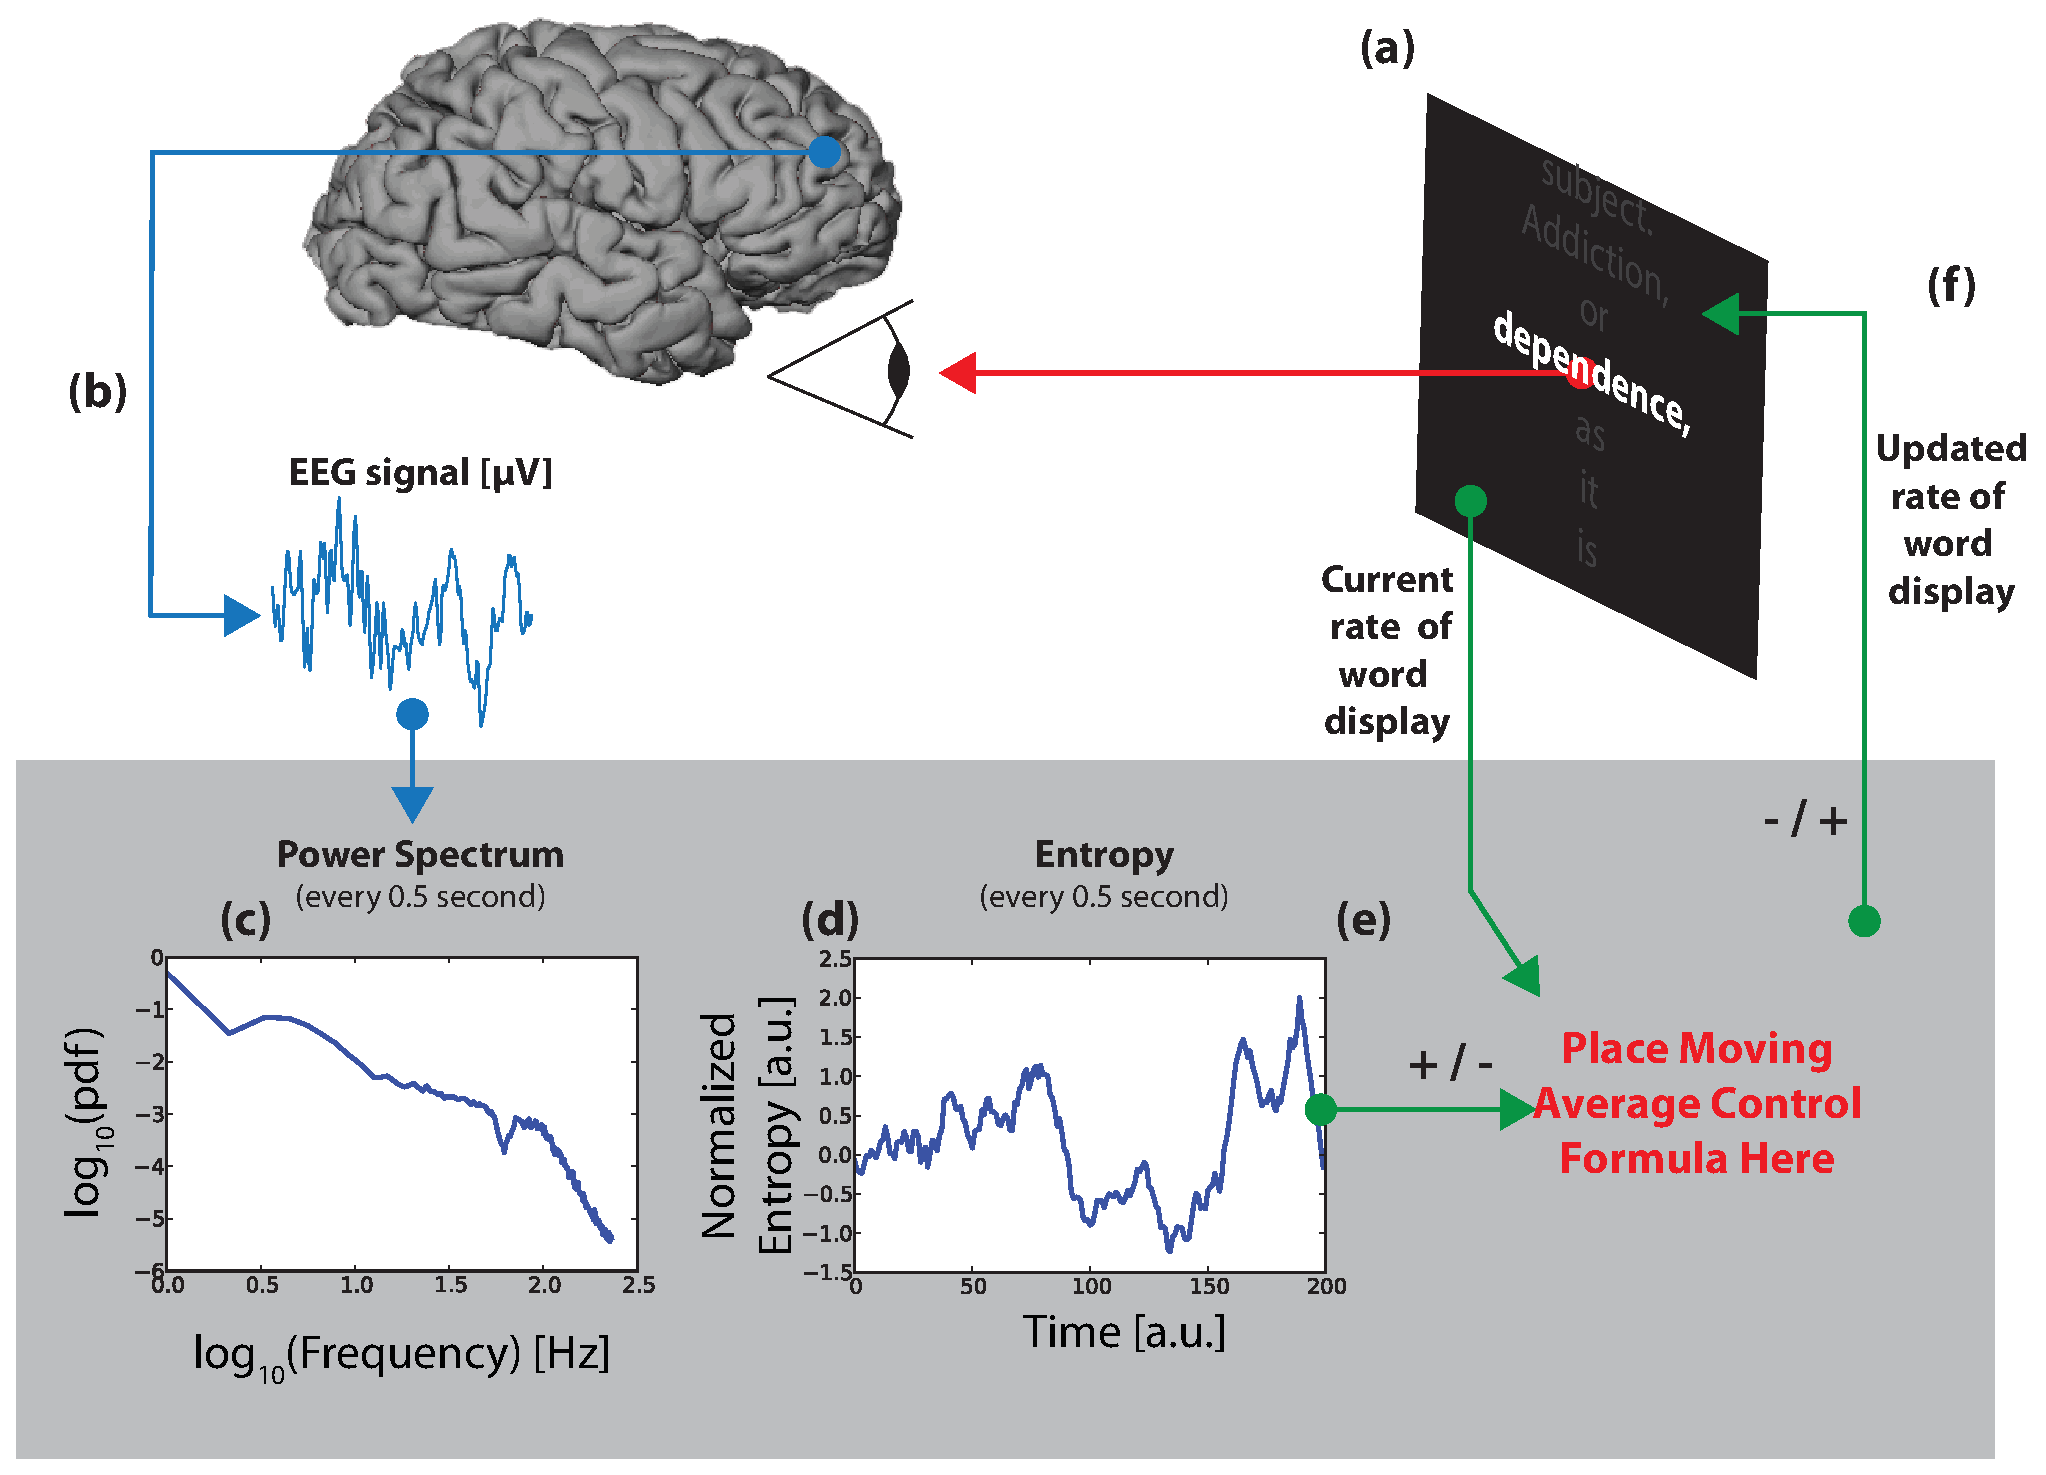
\includegraphics[width=0.9\columnwidth]{../figures/apparatus.eps}
\caption{typical evolution of rate $R$.}
\label{fig:trajectory}
\end{figure}

\section{Experimental Protocol}
To determine the gains of our brain speed-reader apparatus when reading, we have conducted an experiment, involving XX subjects who participated in our study. The experimental procedures described here were approved by an Institutional Review Board. 

\subsection{Procedure}
After obtaining individual consent, we conducted a quick {\bf calibration} task. A text was displayed word by word to each subject, who could adapt the rate of word display with the right (faster) and left (slower) arrow keys, until they reach their comfort zone. This baseline rate would be reused during the experiment. Then, the subject was asked to {\bf wear} the Neurosky Mindset. When ready, a {\bf text was displayed word by word} in a Rapid Visual Serial Presentation (RVSP) manner. After all text was been displayed, the subject was asked some comprehension questions regarding the content of the text. This procedure was repeated three or four times with various texts and various treatments involving varying the rate $R$ of word display:

\begin{enumerate}
  \item {\bf Constant Rate: } the rate of word display remains constant with $R(t) = R_{0}$ for $\forall t$.  
  \item {\bf Brainwave Treatment: } starting from the baseline $R_0$, the rate $R$ changes every quarter second as a function of the rate at the previous step and as a function of the entropy $S_{norm}$ measured in real-time from the EEG captured by the Neurosky mindset, and according to formula (\ref{eq:RateChange}).
    \item {\bf Random Rate Treatment: }  %Randomly Varying Text : R(1) $\rigtharrow$ AR1(n,baseline,baseline/2,0.5,sigma=std) AR1 formula : c + phi * X[-1] + np.random.normal(scale=sigma)
\end{enumerate}

The subject was wearing the Neurosky headset and was not informed whether the treatment involved using EEG as an input for controlling the rate $R$ of word display. In other word, the subject and no information on the three treatments, and had no possibility to distinguish between these treatments, in other ways than guessing from their experience.

In case, four treatments were applied, one of the treatments was repeated once with a different text. After the end, subjects were asked to fill short surveys for each text, asking about comfort, perceived level of understanding, degree of control, followed by a survey to collect demographic informations.

\subsection{Measuring Text Complexity}

ATOS  ( ref: Michael Milone,The Development of ATOS, The Renaissance Readability Formula, p10 (2010) \url{http://doc.renlearn.com/KMNet/R004250827GJ11C4.pdf}

\begin{itemize}
  \item Words per sentence
  \item Average grade level of words ( which class grade the word is first seen)
  \item Characters per word
\end{itemize}


$ATOS Rasch Difficulty Formula = -8.54 + 1.95 * Ln(AvgWords) + .46 * AvgGrad100 + 1.74 * Ln(AvgChar)$

Adjustment for books with less than 500 words

$BLGL for Books With Fewer Than 500 Words = .004 * Book Length + 0.4$


Table detailing texts : \url{https://docs.google.com/spreadsheets/d/1uwkoToM-p3UFrd0U_1vOX4eBJsmYuPVYVhvhsZ8Y5Nc/edit#gid=0}




%\begin{itemize}
%  \item {\bf text 0 (adapted from Coming of Age in Samoa, Margaret Mead, 1928
%)}:   $ATOS=9.5$,  $word~count = 421$
%  \item {\bf Text 1  (adapted from The Warden, Anthony Trollope, 1855)} : $ATOS=8.3$, $word~count = 563$
%  \item {\bf Text 2  (adapted from The Mayor of Casterbridge, Thomas Hardy, 1886) } : $ATOS=10.2$, $word~count = 831$
%  \item {\bf Text 3 (Adapted from: The Social Function of Science, John D Bernal (1939))} : $ATOS=11.9$, $word~count = 421$
%\end{itemize}


\section{Results}
\label{results}


For $17$ over $21$ participants, the RSVP rate was characterized by a balanced joint probability of {\it rate change x word size frequency} in treatment (ii) and (iii) (Fig. 2a). Long words triggered the largest change of entropy (resp. rate), while words smaller than the average size ( $< 5.5$ characters) were associated with reverse entropy (resp. rate) change (Fig. 2b, 2c).\\

Despite the large variation of entropy, texts could be decoded by matching the sequence of entropy measures (associated with each word) with the unique sequence of word lengths (Fig 3). Our results did not require preliminary identification of participants, and the success rate was 27.4\%, roughly 11\% above chance (i.e., $1/6 \approx 16.67\%$), when considering the first 300 words of each text.



\begin{itemize}
  \item performance*, perceived comfort and control as a function of treatment 
  \item for brain speed reader treatment:  performance*, perceived comfort and control as a function $X_0$, $alpha$
\end{itemize}

*performance means either {\bf conceptual} (understanding the meaning), {\bf conceptual-memory} (recalling characters) or {\bf memory} (recalling some words).


\section{Discussion}
\label{discussion}
Recognizing the importance of reading more in less time, while avoiding multi-tasking, we have put to the test the {\it brain speed reader}, a brain-computer interface (BCI) implementing a rate varying rapid serial visual presentation (RSVP) of text words. We have found that a majority of users who participated in our study could control the brain speed reader. Furthermore, we found that roughly half of participants could self-regulate with two opposite control mechanisms ({\it bsr+} and {\it bsr-}). The achievement of self-regulation is negatively influenced by age, text length, topic familiarity and speed reading comfort. Self-regulation achievement (stability) is however highly positively correlated with reading pleasure. Capacity to provide a meaningful text summary {\it ex-post} (the best way to test for text comprehension) is also positively associated with stability, yet in a weakly significant way.

Our results show that the brain speed reader is an adequate technology to foster fast knowledge integration in a world of abundant information and endless news feeds, while at the same time helping preventing multi-tasking. The design implements self-regulation neurofeedback as a way to ensure that users concentrate on reading the text: If the user does not or cannot concentrate, the RSVP rate will drift towards very slow (resp. fast) word display rates. Multi-tasking is discouraged by design, and reading speed is doubled compared to normal reading.

Self-regulation neurofeedback stems from the capacity by the brain to train and adapt its wave modulations in order to perform specific tasks better \cite{piano_neurofeedback}, or to reach desired mental states \cite{neurofeedback_meditation}.  As a special kind of neurofeedback BCI, the brain speed reader may be help remediate reading disabilities or difficulties associated with a lack of concentration capabilities, which is one consequence of multi-tasking. Because the brain speed reader (BSR) does not require prior calibration, training and use occur concomitantly: Either the user achieves self-regulation quickly and then {\it uses} BSR, or she remains in training mode until she reaches self-regulation. In our experiment, we have set very large boundary for slowest (resp. fastest) RSVP rate to make sure that subjects who reach the boundaries effectively failed achieving self-regulation. In training mode, these RSVP rate boundaries may be tuned and personalized to ensure that the user can reach a compromise between attempts to achieve self-regulation and still reading fast with pleasure while training. While we have not tested medical applications for the brain speed reader, it may help users suffering from dyslexia or attention disorder and hyperactivity disorders (ADHD) improve their reading and their attention.

\subsection{Limitations}
The version of the brain speed reader presented here is a first attempt to harness self-regulated neurofeedback for the sake of upgrading the reading experience to arising challenges in society, such as tackling the abundance of natural language- written information while reducing multi-tasking. Although our first experiment show encouraging results, we have come up with the simplest possible implementation and experimental protocol. A number of outstanding questions remain and deserve further work, starting with the hardware we used. Neurofeedback most often involves a limited number of EEG electrodes, but typically of higher quality and on other positions in the 10-20 system. One may want to experiment with a variety of electrode quality, number, and positions to elicit a better hardware configuration.

Our study bears a number of limitations regarding comprehension and memory. We did not find a significant difference of comprehension between RSVP speed read at constant rate versus {\it bsr+} and {\it bsr-} treatments. We find a slight comprehension improvement when users achieve more stable self-regulation, but this result need further validation, presumably with a larger data set. We have also not measured how comprehension and word recall are diminished (resp. increased) as reading speed doubles, i.e., when comparing brain speed reading and reading text normally. Previous research suggests that comprehension is diminished by constant RSVP rate speed reading \cite{kujala2007phase}, although it remains the same or is slightly improved for people with reading disabilities. Further investigation is required to better elicit how self-regulation stability influences comprehension and word recall

We shall also investigate why some participants could not achieve self-regulation: It remains unclear if they had indeed to train further before making it right, or if the BSR parameters we chose [initial RSVP rate $X(t=0) = 125$ ms/word and $|\alpha| = 0.005$] may only be suitable for a subset of the population, and may require further adaptation. Similarly, we have no information on the time it takes to learn given that the user could not achieve self-regulation at once. We chose $X(t=0) = 125$ ms/word as the starting RSVP rate, which is also the value known to be most comfortable on average to people who read with RSVP. To further understand and validate the self-regulation mechanism, it would be desirable to perform additional investigations with a variety of starting rates. Our hypothesis is that within a yet unknown RSVP rate range, users capable of self-regulation can stabilize the rate, while beyond some limits it is impossible to control the brain speed reader, in particular when the presentation speed is high. It also remains to be seen if users tend to stabilize the rate close to 125ms/word on average, even if the initial RSVP rate is smaller (resp. larger).

Even though there is no need for preliminary {\it ad-hoc} calibration to use the brain speed reader, learning still occurs ``on the fly", with several advantages as already mentioned above. It would nevertheless be desirable to better understand how the user transitions from {\it learning} to {\it using}. This has implications for more elaborate and personalized UX design.

Finally, we found that text length has a negative effect on self-regulation stability (roughly one unit per 1300 words as shown in Table \ref{tab:reg}). This is a concern because the brain speed reader is supposed to let users avoid multi-tasking to concentrate on a single task instead. Here, it appears that if the task lasts too long, then self-regulation undergo changes of regime and reduced stability. This suggests that either BSR is suited for {\it long but not that long tasks} and/or there is another factor involving learning how to keep self-regulation highly stable over long tasks. This is has further implications on comprehension and memory, which need to be further addressed.

\subsection{Beyond speed reading}
Here, we have designed and tested brain-computer interface (BCI), which helps seamlessly control the parsing rate of a coherent sequence of a words as visual stimuli. The same time varying rate RSVP coupled with a neurofeedback BCI may be used beyond reading. It could apply similarly to cartoons, video or audio streams, if the control is made on the continuous speed (i.e., the pitch) of the media stream, similarly to the (discrete) presentation rate used in our experiment.

Similar BCI could be used to assess the quality and the coherence of a piece of text. Indeed, it appears that when reading, the brain makes some heuristic predictions of what word(s) is (resp. are) coming next \cite{smith2013effect}. Unexpected words trigger an unusual cognitive activity which slows the reading. Recording how the effects of unexpected stimuli materialize in conjunction with control remain yet to the be investigated. 

\section{Future Work}

\bibliographystyle{abbrv}
%\bibliography{bib/tmaillart.bib,bib/references.bib}


\end{document}
